\chapter{Способ построения Актор-Критик САУ} \label{chapt2}

В подходе с обучением с подкреплением целью функционирования агента является максимизация целевой функции, который представляет собой суммарную величину награды - подкрепления. Такого типа управление относится к классу систем экстремального управления (СЭУ).

\section{Структурная схема системы экстремального управления} \label{sect2_1}
Системы экстремального управления относят к классу адаптивных систем, такие системы отличаются автоматическим выбором режима управления, при котором поддерживается минимальное или максимальное значение некой целевой функции. 

\begin{figure}[ht] 
  \center
  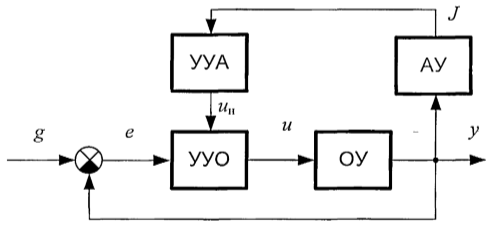
\includegraphics [scale=1] {seu_21}
  \caption{Структурная схема СЭУ} 
  \label{img:seu_21}  
\end{figure}

%\newpage
%============================================================================================================================
\section{Структурная схема Актор-Критик САУ} \label{sect2_2}
С помощью метода Актор-Критик и обучения с подкреплением разработана обобщенная структурная схема Актор-Критик САУ, изображенная на рисунке ~\ref{img:ac_struct}, а также алгоритмы функционирования системы
\begin{figure}[ht] 
	\center
	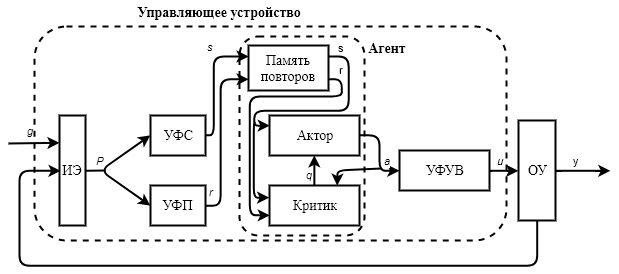
\includegraphics [scale=0.7] {ac_struct}
	\caption{Структурная схема Актор-Критик САУ} 
	\label{img:ac_struct}  
\end{figure}


Объект управления должен обладать свойствами частично наблюдаемого марковского процесса (POMDP)

\subsection{Импульсный элемент} \label{subsect2_2_1}
Целью функционирования импульсного элемента является дискретизация поступающего на вход сигнала с шагом $\tau_{\text{УУ}}$, который является параметром настройки УУ. ИЭ отвечает за формирование вектора дискретных сигналов $\bar{P}[k]$, который вектор поступает на входы УФС и УФП. Вектор $\bar{P}[k]$ состоит из $N_{\text{ОУ}}$ элементов, где $N_{\text{ОУ}}$ количество переменных состояния ОУ.

\subsection{Устройство формирования состояния} \label{subsect2_2_2}
Блок УФС отвечает за создание вектора состояний $s[k]$, который поступает на вход Актору и Критику. Данный вектор состоит из квантованных и нормализованных к масштабу [-1, 1] значений вектора $\bar{P}[k]$. Нормализация к данному масштабу объяснятся отраслевым стандартом.

\subsection{Устройство формирования подкрепления} \label{subsect2_2_3}

УФП отвечает за выработку сигнала подкрепления $ r[k] $ из вектора дискретных значений $ \bar{P}[k] $ c помощью функции $ f $:
$$
r[k] = f(p_1[k]), p_2[k]), p_{N_p}[k])).
$$

Данная функция является параметром настройки блока УФП, и выбирается в зависимости от задачи. Если целью функционирования системы является поддержание некого постоянного значения $ y_{\text{зад}} $, то функция вычисления сигнала подкрепления может иметь вид:

$$
f(y) = -(y-y_{\text{зад}})^2.
$$

\noindent Такой вид функции обеспечивает максимальный сигнал подкрепления (равный 0) только в том случае, если значение выходного сигнала совпадет с  $ y_{\text{зад}} $.

Когда целью функционирования системы является достижение единовременное некоторой цели, например передвижение кибер-физической системы из одного положение в другое, то функций расчета подкрепления становится система эвристических правил. Например, задачей мобильного робота является перемещение из положения $ A $ в положение $ A^* $, а положение самого робота обозначается $ A_r $. Функция $ D_{(A^*, A_r)} $ расчитывает расстояние между мобильным роботом и целевой точкой. Функция расчета сигнала подкрепления может иметь следующий вид:

$$
r[k] = 
\begin{cases}
1, \: \text{если} \: D_{(A^*, A_r)}=0; \\
0.1, \: \text{если} \: D_{(A^*, A_r)}[k] < D_{(A^*, A_r)}[k-1]; \\
-0.1 \: \text{иначе}.
\end{cases}
$$

\noindent В данной функции отрицательное подкрепление или штраф агент получает в случае бездействия, когда расстояние до цели не уменьшается, награждается в случае сближения с целью, и самый большой сигнал подкрепления агент получает в случае попадания в цель.

На практике вводится некоторая отсечка $ T_{\text{сближ}} $ для расчета сигнала подкрепления в случае сближения робота с целью, если величина сближения  меньше этой отсечки, то награда не назначается. Это делается для исключения колебаний сигнала подкрепления. Дополнительно вводится отсечка достижения робота цели $ T_{\text{цели}} $. Если робот слишком далеко переместился от цели, дальше чем $ T_{\text{откл}} $, то назначается штраф. После введения вышеперечисленных отсечек функция расчета подкрепления принимает следующий вид:

$$
r[k] = \begin{cases}
1, \: \text{если} \: D_{(A^*, A_r)} < T_{\text{цели}}; \\
0.1, \: \text{если} \: D_{(A^*, A_r)}[k-1] - D_{(A^*, A_r)}[k] > T_{\text{сближ}}; \\
-1 \: D_{(A^*, A_r)} > T_{\text{откл}};\\
-0.1 \: \text{иначе}.
\end{cases}
$$

\noindent Данные отсечки являются параметрами настройки блока УФП. Если сигнал подкрепления равен 1 или -1 то эпизод заканчивается победой или поражением соответственно.

\subsection{Агент} \label{subsect2_2_4}
"Агент" является блоком, реализующим алгоритм, в основе функционирования которого лежит метод Актор-Критик. Данный метод был выбран на основе анализа, приведенного в главе \ref{subsect1_3_6}.

На вход данного блока подается вектор состояния $s[k]$ и сигнал подкрепления $r[k]$. Блок "Агент" состоит из трёх подблоков: Актора, Критика и блока повторов. Актор отвечает за формирование сигнала управления и Критик за анализ качества управления. Блок повторов содержит в себе информацию о предыдущих результатах взаимодействия Актора, Критика и средой. У <<Агента>> есть два режима функционирования:
\begin{enumerate}
	\item Обучение. Задействованы и Актор и Критик.
	\item Предсказание. Работает только Актор.
\end{enumerate} 

Параметрами настройки блока <<Агент>> являются:
\begin{itemize}
	\item $ N_s $ - количество состояний $s[k]$;
	\item $ N_a $ - количество параметров во множестве воздействий на ОУ $ A $;
	\item $ \gamma $ - коэффициент дисконтирования сигнала подкрепления;
	\item $ \Delta $ - коэффициент скорости обучения (learning rate);
	\item $ f_{\epsilon} $ - закон изменения коэффициента исследования;
	\item $ N_R $ - количество элементов в памяти повторов;
	\item также в качестве параметров настройки блока выступают количество слоев ИНС и количество нейронов в каждом из них.
\end{itemize}
 
Подблоки Актор и Критик использует для аппроксимации своих функций глубокие нейронне сети (DNN - deep neural network), настраиваемыми параметрами которых являются $ \theta_A $ и $ \theta_K $ соответственно. Метод, которым производится обучение Актора и Критика называется DDPG (Deep deterministic policy gradient). 

Функция Критика аппроксимируется через минимизацию квадратичной ошибки временной разности:

$$
L(\theta_K) = (r_{i+1} + \gamma Q(s_{i+1}, \pi(s_{i+1}|\theta_A)|\theta_K) - Q(s_i, a_i|\theta_K))^2
$$

$$
y_i = r_i + \gamma Q'(s_{i + 1}, \mu'(s_{i+1}|\theta^{\mu'})|\theta^{Q'})
$$

$$
L = \frac{1}{N} \sum_{i} (y_i - Q(s_i, a_i | \theta^{Q})^2) 
$$

$$
\nabla_{\theta^{\mu}} \mu \approx \mathbb{E}_{\mu'} \big [ \nabla_{a} Q(s, a|\theta^{Q})|_{s=s_t,a=\mu(s_t)} \nabla_{\theta^{\mu}} \mu(s|\theta^{\mu})|_{s=s_t} \big ]
$$

Веса нейронной сети Актора настраиваются по направлению градиентов $ \Delta Q_{\theta_A} $ по следующей формуле:

$$ 
\Delta \theta_A = \Delta
$$

$$
a[k] = 
\begin{cases}
a^*[k], \: \text{если} \: e \geq \epsilon  \\
a_t, \: t=[rand \cdot N_a]
\end{cases}
$$

Алгоритм работы блока <<Агент>>:
\begin{enumerate}
	\item В соответсвии с () $ \epsilon $ - жадной стратегии выбирается действие $ a_i $ для текущего состояния $ s_i $.
	\item Считывается следующее состояние $ s_{i+1} $ и награда $ r $
	\item Кортеж $ a_i $, $ s_i $, $ s_{i+1} $ и $ r $ записываются в подблок <<Память повторов>>
	\item Считывается N записей из подблока <<Память повторов>>
	\item На основании () производится обновление весов нейронной сети Критика
	\item На основании () производится обновление весов нейронной сети Актора
\end{enumerate}

\subsection{Устройство формирования управляющего воздействия} \label{subsect2_2_5}
Данное устройство предназначено за преобразование предсказанного "Агентом" действие в управляющее воздействие для конкретного ОУ.


\section{Экспериментальные исследования Актор-Критик САУ} \label{sect2_3}

\subsection{Управление машиной Дубинса в задаче преследования} \label{subsect2_3_1}

$ R $ - ОУ, робот

$ M $ - цель

$ O_1, O_2 $ - препятствия

$ y $ - вектор состояния робота

$$
\begin{cases}
y_1 = \rho_1(R, O_1, O_2) \\
y_2 = \rho_2(R, O_1, O_2) \\
y_3 = \rho_3(R, O_1, O_2) \\
y_4 = \rho_c(R, M)
\end{cases}
$$
\newpage
$ \rho_1 - \rho_3 \in [d_{min}, d_{max}] $ - функции дальномеров 

где $ d_{min}, d_{max} $ - мин и мак дальности измерений


Цель - максимизировать совокупную награду:
$$
r[k] = \begin{cases}
1, \: \text{если} \: D_{(M, R)} < T_{\text{цели}}; \\
0.1, \: \text{если} \: D_{(M, R)}[k-1] - D_{(M, R)}[k] > T_{\text{сближ}}; \\
-1 \: D_{(M, R)} > T_{\text{откл}};\\
-0.1 \: \text{иначе}.
\end{cases}
$$



\noindent$ D $ - функция, рассчитывающее расстояние.

\noindent$ T_{\text{цели}} $ - отсечка расстояния до цели,\\
меньше которой цель считается захваченной.

\noindent$ T_{\text{откл}} $ - отсечка, при превышении которой\\
считается, что робот уходит от цели.

\noindent$ T_{\text{сближ}} $ - отсечка, меньше которой\\
считается, что робот уходит от цели.

Уравнение движения робота
$$
\begin{cases}
\frac{dx_R}{dt} = f_1(R, u, \phi) \\
\frac{dy_R}{dt} = f_2(R, u, \phi) 
\end{cases}
$$

\noindent$ u \in [u_{left}, u_{forward}, u_{left}]$ - управляющее воздействие на робота\\
\noindent $ \phi $ - минимальный радиус поворота\\

Среда (рис. ), в которой действует мобильный робот (охотник) представляет собой поле шириной 1000 пикселей и высотой 700. Робот представляет собой машину Дубинса, кинематические свойство которого описываются системой уравнений (\ref{eq:2_3_1p1}). В среде находятся жертва, препятствия и мобильный робот. Задача робота приблизится к жертве на расстояние не меньше 0.5 метра (что соответствует 100 пикселям на экране) относительно центра жертвы, при этом не задев препятствия и границы среды. У мобильного робота есть 4 сенсора: 3 сонара и компас, который показывает относительный угол между осью движения мобильного робота и центром жертвы. Управление мобильным роботом осуществляется посредством выбора одной из трёх команд: “налево”, “прямо”, “направо”. Управление скоростью робота не предполагается в данной задаче. Инициализация робота происходит всегда в одной позиции, но угол каждый раз выбирается случайно. Также, среда поддерживает режим, при котором жертва может двигаться случайно по плоскости.

\begin{equation}
	\label{eq:2_3_1p1}
	\left\{
	\begin{alignedat}{2}
	\frac{dx}{dt}=v\cdot \cos (\phi ) \\
	\frac{dy}{dt}=v\cdot \sin (\phi ) \\
	\frac{d\phi}{dt}=\frac{\pi}{2}(u_{rm}-u_{lm}) \\
	v=0.5(u_{rm}-u_{lm})
	\end{alignedat}
	\right.
	\text{где}
	\left\{
	\begin{alignedat}{2}
	u_{rm}=[0,1]\\
	u_{lm}=[0,1]
	\end{alignedat}
	\right.
\end{equation}

\begin{figure}[ht] 
	\center
	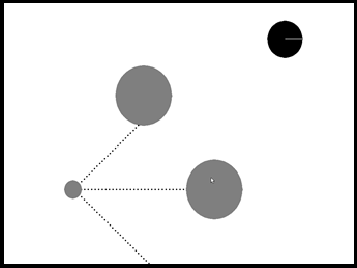
\includegraphics [scale=1] {dubins/image14.png}
	\caption{Визуализация среды, объекты: маленький серый - хищник, белые точки - линии действия сонаров, два больших серых - препятствия, белый-жертва} 
	\label{img:dubins}  
\end{figure}

Тестирование проводилось для случаев со статической жертвой, со стохастической жертвой, при котором жертва выбирала направление движения случайно, а также с убегающей жертвой, при котором жертва всегда убегает под углом +/-90$ {^\circ} $ относительно приближающегося хищника. 
И в случае со стохастической жертвой и с убегающей скорость жертвы равна скорости хищника. 
Также, тестирование проводилось для случаев с минимальными радиусами разворота машины Дубинса равными 50 и 100 пикселей. Качество агента сравнивалось с жадным алгоритмом, его схема работы:

\begin{enumerate}
	\item Если угол до цели меньше -3$ {^\circ} $, то выбираем поворот налево. Если угол больше 3$ {^\circ} $, то выбираем поворот направо. В остальных случаях выбираем движение прямо
	\item Если расстояние до препятствия по данным левого сонара меньше 100 пикселей, то выбираем поворот направо. Если расстояние до препятствия по данным правого и центрального сенсора меньше 100 пикселей, то выбираем поворот налево
\end{enumerate}

\begin{figure}[ht] 
	\center
	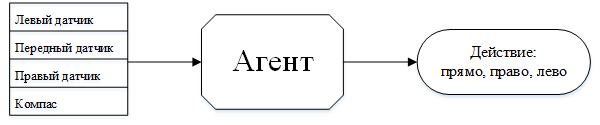
\includegraphics [scale=1] {dubins/image25.png}
	\caption{Схема работы Актор-Критик САУ для управления мобильным роботом} 
	\label{img:dubins2}  
\end{figure}

\begin{table} [htbp]
	\centering
	\caption{ Архитектуры ИНС Актора и Критика }
	\label{Ts0Sib1}%
	\begin{tabular}{| p{1cm} || p{6cm} | p{6cm} l|}
		\hline
		\hline
		& \centering Актор & \centering Критик  & \\
		\hline
		1 &\centering  Полносвязный: 256 &\centering Полносвязный: 256& \\
		2 &\centering  Дропаут: 20\% & \centering Дропаут: 20\% & \\
		3 &\centering  РЕЛУ  &\centering  РЕЛУ    &   \\
		4 &\centering  Полносвязный: 256 &\centering  Полносвязный: 256 &   \\
		5 &\centering  Дропаут: 20\% &\centering  Дропаут: 20\%  &   \\
		6 &\centering  РЕЛУ   &\centering  РЕЛУ    &   \\
		7 &\centering  Полносвязный: 3 &\centering  Полносвязный: 1  &   \\
		\hline
		\hline
	\end{tabular}
\end{table}

Качество агента оценивалось как доля успешных запусков, то есть случаев, когда машина поймала жертву. В таблице 2 приведены результаты тестирования жадного алгоритма и модели Актор-Критик, которое проводилось на 1000 повторений. На рис. 4 представлены примеры траекторий для жадного алгоритма и метода Актор-Критик.

\begin{figure}[ht]
	\begin{minipage}[ht]{0.49\linewidth}\centering
		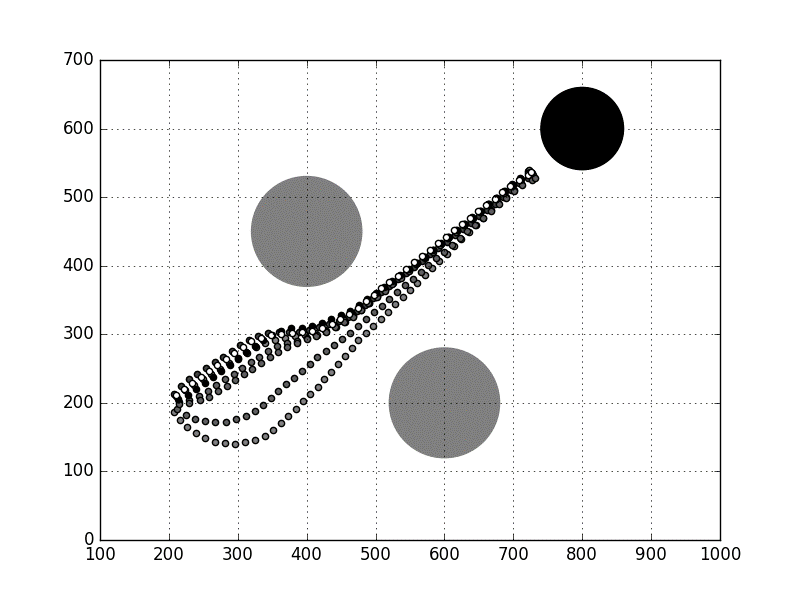
\includegraphics[width=1\linewidth]{dubins/image15.png} \\ а)
	\end{minipage}
	\hfill
	\begin{minipage}[ht]{0.49\linewidth}\centering
		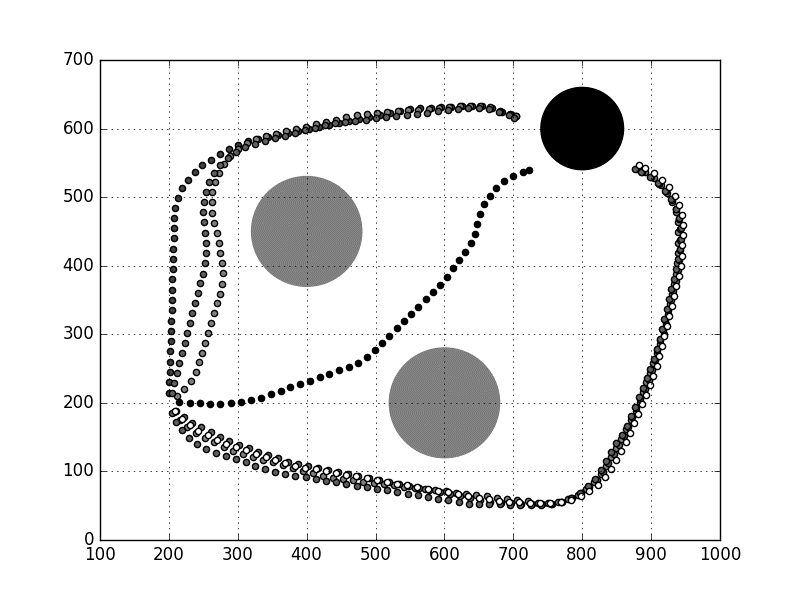
\includegraphics[width=1\linewidth]{dubins/image16.png} \\ б)
	\end{minipage}
	\caption{Статическая жертва, слева - траектория при жадном алгоритме, справа - Актор-Критик метод}
	\label{img:knuth}  
\end{figure}

\begin{table} [htbp]
	\centering
	\caption{ Доли успешных запусков для жадного алгоритма и модели Актор-Критик }\label{Ts0Sib}%
	\begin{tabular}{| p{6cm} || p{4.5cm} | p{2.5cm} l|}
		\hline
		\hline
		Режим работы    & \centering Жадный Алгоритм & \centering АКСАУ  & \\
		\hline
		Статическая/радиус 50 &\centering  0.372   &\centering  0.788    &\   \\
		Динамическая/радиус 100  &\centering  0.832   &\centering  0.911    &\   \\
		Статическая/радиус 50 &\centering  0.399  &\centering  0.735    &   \\
		Динамическая/радиус 100 &\centering  0.757  &\centering  0.762    &   \\
		Статическая/радиус 50 &\centering  0.370   &\centering  0.766    &   \\
		Динамическая/радиус 100 &\centering  0.697   &\centering  0.758    &   \\
		\hline
		\hline
	\end{tabular}
\end{table}

Как видно в таблице (), во всех случаях метод Актор-Критик выигрывает, в некоторых случаях совсем немного, а в некоторых – существенно.

\subsection{Управление настройками ПИ-регулятора в задаче управления двуосным прокатным станом} \label{subsect2_3_2}

Двуосный прокатный стан (ДПС) является многомерной многосвязной системой. Приложение управляющего воздействия на одну из осей \textit{u${}_{x}$${}_{, }$}или\textit{${}_{ }$u${}_{y}$} влияет на другую ось. Управление осями осуществляется подачей двух управляющих воздействий. Имеются датчики давления волков по каждой из оси (\textit{f${}_{x}$${}_{, }$f${}_{y}$}), а также показания датчиков, которые осуществляют контроль отклонения толщины металла от заданной величины ($\delta _{x} $${}_{,}$${}_{ }$$\delta _{y} $). Необходимо осуществить управление таким образом, чтобы минимизировать функцию стоимости при действии возмущающих воздействий в в виде:   
$$
C(u)=\int _{0}^{\infty }(\delta ^{2} (t)+\beta u^{2} (t))dt,^{} \beta  =0.0001
$$

\begin{figure}[ht] 
	\center
	\includegraphics* [scale = 0.7, keepaspectratio=false, trim=1.79in 1.83in 7.69in 1.35in] {DPS/image6}
	\caption{Модель ДПС} 
	\label{img:agent_dps1}  
\end{figure}

\begin{figure}[ht] 
	\center
	\includegraphics* [scale = 0.7, keepaspectratio=false, trim=0.67in 1.71in 3.57in 1.12in] {DPS/image7}
	\caption{Подмодель оси х} 
	\label{img:agent_dps2}  
\end{figure}

Описание ДПС в виде дискретных передаточных функций:

$$F_{ex} =\frac{a_{1} z+a_{0} }{b_{2} z^{2} +b_{1} z+b_{0} } ,$$ где $a_{1} =30,_{} a_{0} =-30,_{} b_{2} =1,_{} b_{1} =-2,_{} b_{0} =0.9999$ - изменение эксцентриситета оси \textit{х}

$$F_{ey} =\frac{a_{1} z+a_{0} }{b_{2} z^{2} +b_{1} z+b_{0} } ,$$ где $a_{1} =99.99,_{} a_{0} =-99.99,_{} b_{2} =1,_{} b_{1} =-2,_{} b_{0} =0.9998$ - изменение эксцентриситета оси \textit{у}

$$F_{ix} =\frac{a_{0} }{b_{1} z+b_{0} } ,$$ где $a_{0} =10,_{} b_{1} =1,_{} b_{0} =-1$ - вариация толщины на входе оси \textit{x}

$$F_{iy} =\frac{a_{0} }{b_{1} z+b_{0} } ,$$ где $a_{0} =20,_{} b_{1} =1,_{} b_{0} =-1$ - вариация толщины на входе оси \textit{y}

$$H_{x} =\frac{a_{1} z+a_{0} }{b_{2} z^{2} +b_{1} z+b_{0} } ,$$ где $a_{1} =117.1,_{} a_{0} =114.3,_{} b_{2} =1,_{} b_{1} =-1.923,_{} b_{0} =0.9305$ - передаточная функция актюатора оси \textit{х}

$$H_{y} =\frac{a_{1} z+a_{0} }{b_{2} z^{2} +b_{1} z+b_{0} } ,$$ где $a_{1} =380.7,_{} a_{0} =371.8,_{} b_{2} =1,_{} b_{1} =-1.924,_{} b_{0} =0.9315$ - передаточная функция актюатора оси \textit{х.      }Шаг дискретизации $T=0.001$

Формирование награды: $$r(t)=\left\{\begin{array}{c} {0_{} \left|E(t)\right|\le \left|E(t-1)\right|} \\ {-0.5} \end{array}\right. $$ где $E(t)=(\delta ^{2} (t)+\beta u^{2} (t))_{} \beta =0.0001$


\begin{figure}[ht] 
	\center
	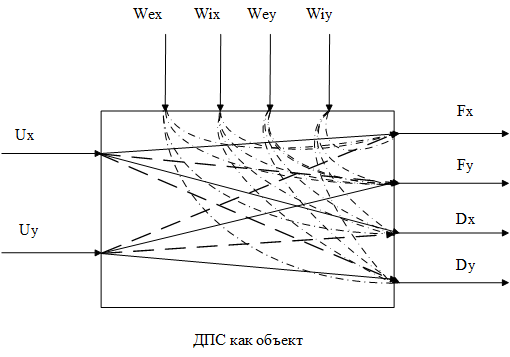
\includegraphics [scale=1] {dps}
	\caption{Представление ДПС как объекта} 
	\label{img:dps}  
\end{figure}

\begin{figure}[ht] 
	\center
	\includegraphics* [scale = 0.7, keepaspectratio=false, trim=0.90in 2.00in 5.09in 1.28in] {DPS/image8}
	\caption{Симулинк модель управления ДПС} 
	\label{img:agent_dps3}  
\end{figure}

\begin{figure}[ht] 
	\center
	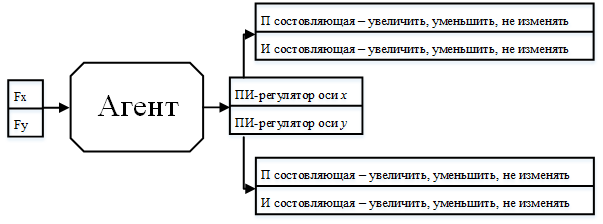
\includegraphics [scale=1] {agent_dps}
	\caption{Структурная схема работы Агента для управления ДПС} 
	\label{img:agent_dps}  
\end{figure}

\begin{table} [htbp]
	\centering
	\caption{ Архитектуры ИНС Актора и Критика }
	\label{Ts0Sib3}%
	\begin{tabular}{| p{1cm} || p{6cm} | p{6cm} l|}
		\hline
		\hline
		& \centering Актор & \centering Критик  & \\
		\hline
		1 &\centering  Полносвязный: 256 &\centering Полносвязный: 256& \\
		3 &\centering  РЕЛУ  &\centering  РЕЛУ    &   \\
		4 &\centering  Полносвязный: 256 &\centering  Полносвязный: 256 &   \\
		6 &\centering  РЕЛУ   &\centering  РЕЛУ    &   \\
		7 &\centering  Полносвязный: 3 &\centering  Полносвязный: 1  &   \\
		\hline
		\hline
	\end{tabular}
\end{table}


\begin{table} [htbp]
	\centering
	\caption{ Доли успешных запусков для жадного алгоритма и модели Актор-Критик }\label{Ts0Sib2}%
	\begin{tabular}{|p{1.3in}|p{1.3in}|p{1.3in}|p{1.3in}|p{1.3in}|} \hline 
		& \multicolumn{2}{|p{2.7in}|}{ДПС модель без изменений\newline в $H_{x} $$b_{1} =-1.923$\newline в $H_{y} $$b_{1} =-1.924$} & \multicolumn{2}{|p{2.7in}|}{в $H_{x} $$b_{1} =-1.823$\newline в $H_{y} $$b_{1} =-1.824$} \\ \hline 
		& Референс & Актор-Критик агент & Референс & Актор-Критик агент \\ \hline 
		$C(u)$[x, y] & \textbf{[0.97 0.37]} & [1.45 1.45] & [12.26 16.97] & \textbf{[1.83 0.89]} \\ \hline 
		$\delta _{x} $[min, max] & [-0.15 0.12] & [-0.23 0.37] & [-0.75 0.55] & [-0.25 0.41] \\ \hline 
		$\delta _{y} $[min, max] & [-0.16 0.12] & [-0.22 0.39] & [-0.49 0.44] & [-0.19 0.31] \\ \hline 
	\end{tabular}
\end{table}

\section{Основные выводы по главе 2} \label{sect2_4}

\begin{enumerate}
	\item Приведено описание схемы Актор-Критик САУ, использующей в своей основе глубокие нейронные сети для аппроксимаций функций Актора и Критика.
	\item Приведено описание алгоритмов работы каждого блока схемы Актор-Критик САУ
	\item Приведено описание разработанного программного средства для моделирования работы Актор-Критик САУ в различных конфигурациях с разными средами.
	\item Приведены результаты экспериментальных исследований, в процессе которых изучалось применение Актор-Критик САУ для различных объектов управления.
\end{enumerate}




\newpage

$ R_i, R_j $ - ОУ, два робота

$ M_i, M_j $ - две цели

$ y $ - вектор состояния каждого робота

$$
\begin{cases}
y_1 = \rho_1(R) \\
y_2 = \rho_2(R) \\
y_3 = \rho_3(R) \\
y_4 = \rho_c(R, M_i, M_j)\\
y_5 = w
\end{cases}
$$
\newpage
$ \rho_1 - \rho_3 \in [d_{min}, d_{max}] $ - функции дальномеров 

где $ d_{min}, d_{max} $ - мин и мак дальности измерений

$ \rho_c $ - функция компаса, показывающего угол до цели

$ w $ - номер слова, произнесенного другим роботом


Цель - максимизировать совокупную награду:
$$
r_i[k] = \begin{cases}
1, \: \text{если} \: D_{(M_i, M_j, R_i, R_j)}^* < T_{\text{цели}}; \\
0.1, \: \text{если} \: D_{(M_i, R_i)}[k-1] - D_{(M_i, R_i)}[k] > T_{\text{сближ}}; \\
-1 \: D_{(M_i, R_i)} > T_{\text{откл}};\\
-0.1 \: \text{иначе}.
\end{cases}
$$



\noindent$ D $ - функция, рассчитывающее расстояние.

\noindent$ D^* $ - функция, рассчитывающее расстояние\\
для нескольких роботов и целей.

\noindent$ T_{\text{цели}} $ - отсечка расстояния до цели,\\
меньше которой цель считается захваченной.

\noindent$ T_{\text{откл}} $ - отсечка, при превышении которой\\
считается, что робот уходит от цели.

\noindent$ T_{\text{сближ}} $ - отсечка, меньше которой\\
считается, что робот уходит от цели.

Уравнение движения робота
$$
\begin{cases}
\frac{dx_R}{dt} = f_1(R, u, \phi, w) \\
\frac{dy_R}{dt} = f_2(R, u, \phi, w) 
\end{cases}
$$

\noindent$ u \in [u_{left}, u_{forward}, u_{left}]$ - управляющее воздействие на робота\\
\noindent $ \phi $ - минимальный радиус поворота\\
